\chapter{Grundlagen}
\label{chapter_Grundlagen}

Bei der Entwicklung des Teststandes kommen verschiedene Systeme, Schnittstellen und Konzepte zum Einsatz. Die Grundlagen dazu werden im folgenden Kapitel kurz erläutert.

\section{QT}
QT ist eine umfangreiche C++-Klassenbibliothek zur Gestaltung und Entwicklung von Anwendungen.Vor allem bei Applikationen mit grafischen Benutzeroberflächen (englisch: \ac{GUI}) ist QT sehr beliebt. \\
Zusätzlich bringt QT eine große Auswahl an Tools und Modulen mit sich, welche die Programmierung erheblich erleichtern (z.B. Netzwerkprogrammierung, Datenbankanbindung, OpenGL, etc.). \\
Ein weiterer Vorteil ist die Plattformunabhängigkeit. So unterstützt QT aktuell (Version 5.4, 10. Dezember 2014) einen Großteil der aktuellen Betriebssystem wie Windows, Linux, Android, iOS und einige mehr.
\\\\
Als Entwicklungsumgebung (englisch: \ac{IDE}) dient der QT Creator (siehe Abbildung \ref{QTCreator}), welcher Teil des \ac{SDK} von QT ist und sowohl auf Linux, Windows und auch Mac OS X zur Verfügung steht. Er kommt mit einem Debugger, einem integrierten grafischen \ac{GUI} Designer und einem Texteditor mit Funktionen wie Syntax-Hervorhebung und automatischer Vervollständigung. \\
Es können alle gängigen Compiler verwendet werden und es besteht die Möglichkeit eigene Toolchains anzulegen. 

\begin{figure}[h]
\begin{center}
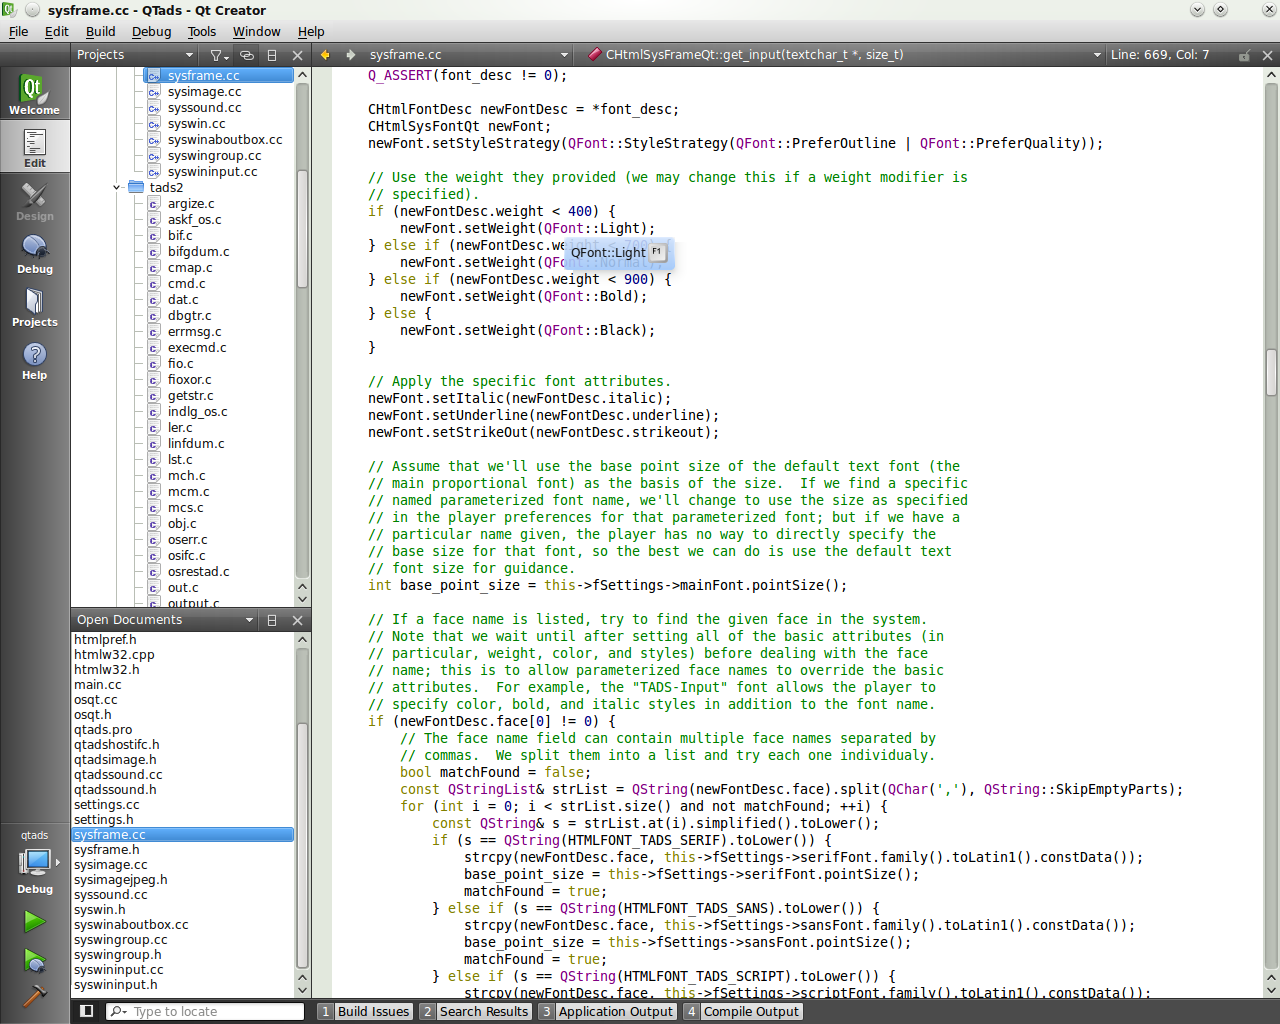
\includegraphics[width=\textwidth]{img/general/QtCreator.png}
\caption{QtCreator Version 2.0.1}
\label{QTCreator}
\end{center}
\end{figure}
\newpage
%Quellen:\\
%http://de.wikipedia.org/wiki/Qt_%28Bibliothek%29
%http://www.mathematik.uni-ulm.de/sai/ws02/cpp/070103/Qt.pdf
%http://wiki.ubuntuusers.de/Qt
%http://en.wikipedia.org/wiki/Qt_Creator

\section{RS232}
Bei RS232 handelt es sich um eine serielle Schnittstelle zu Datenübertragung.

\section{Datenbank}
\label{section_Datenbank}

Für das Speichern der Messdaten und Betriebsparameter wird eine \ac{SQL} Datenbank verwendet. Bei der Wahl des Datenbankverwaltungssystems, standen mehrere Optionen zur Auswahl und die Entscheidung wurde zwischen SQLite und MySQL gefällt.
Beide System haben ihre Vor- und Nachteile.


\textbf{SQLite} ist ein \ac{SQL} Datenbankverwaltungssystem, welches ohne einen Server auskommt und operiert stattdessen in einer einzigen Datei. Es wird vor allem im Embedded Bereich eingesetzt, da kaum Konfigurationen oder Verwaltung notwendig ist. Deshalb eignet es sich ausgezeichnet für sich schnell weiterentwickelnde Applikationen.
\\
Aufgrund dieser Eigenschaften existieren allerdings auch Nachteile. So unterstützt SQLite nur eingeschränkt mehrere Nutzer gleichzeitig. Da das gesamte Datenbanksystem in einer einzigen Datei zusammengefasst ist, können mehrere zur selben Zeit durchgeführte Schreibzugriffe nicht unterstützt werden. Denn die einzige Sicherstellung der Datenintegrität erfolgt durch das Betriebssystem. 
\\
Des Weiteren ist SQLite aufgrund des Ein-Datei-Systems nur eingeschränkt skalierbar. Bei einer größeren Datenmenge oder erhöhten Anzahl an Zugriffen ist es nicht möglich diese Datei auf mehrere Systeme zu separieren, um somit die Last gleichmäßig zu verteilen.

\textbf{MySQL} ist ein weiteres \ac{SQL} Datenbankverwaltungssystem, welches allerdings auf einer Serverarchitektur beruht. 
Es ermöglicht die Verwaltung von Nutzern und Rechte. Außerdem ist das System gut hinsichtlich Performance und Größe zu skalieren. Zusätzlich bietet MySQL viele Möglichkeiten für Performanceanpassungen, wie z.B. Query-Caching.
\\
Jedoch gibt es auch hier Nachteile. So ist die Konfiguration wesentlich schwerer und komplexer. Durch die Notwendigkeit eines Servers benötigt MySQL mehr Ressourcen auf dem Host-System.

Die Wahl fällt auf das relationale Datenbankverwaltungssystem MySQL. Auch wenn SQLite einige Vorteile vor allem im Embedded Bereich besitzt, ist die fehlende Unterstützen von mehreren Nutzern gleichzeitig ein Ausschlusskriterium.

\cite{saake2010datenbanken}